\section{Use-Cases}
\begin{figure}[b]
  \centering
  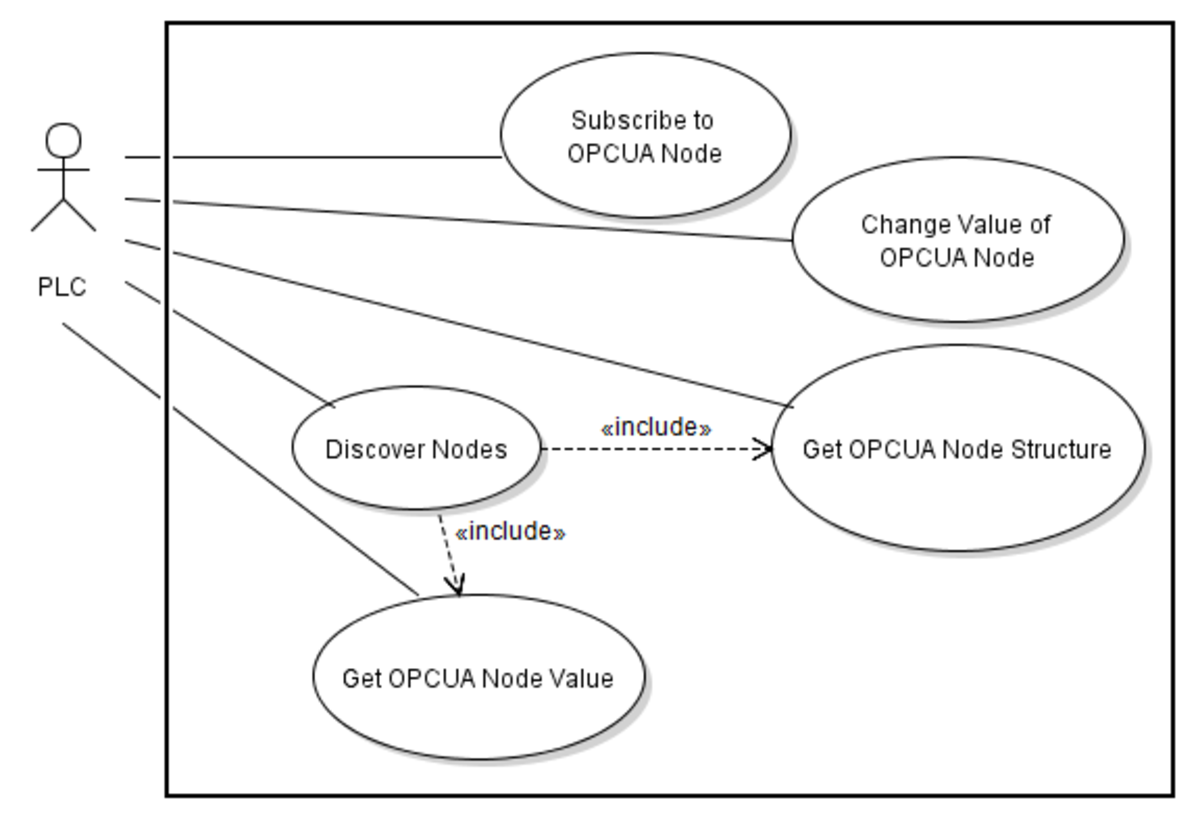
\includegraphics[width=0.82\textwidth]{content/hauptteil/systemEntwurf/res/useCase/II.pdf}
  \caption[Use-Case Diagramm des \acs{scada} Systems II]{Use-Case Diagramm des \acs{scada} Systems II}
  \label{fig:UCII}
\end{figure}

\begin{figure}[b]
  \centering
  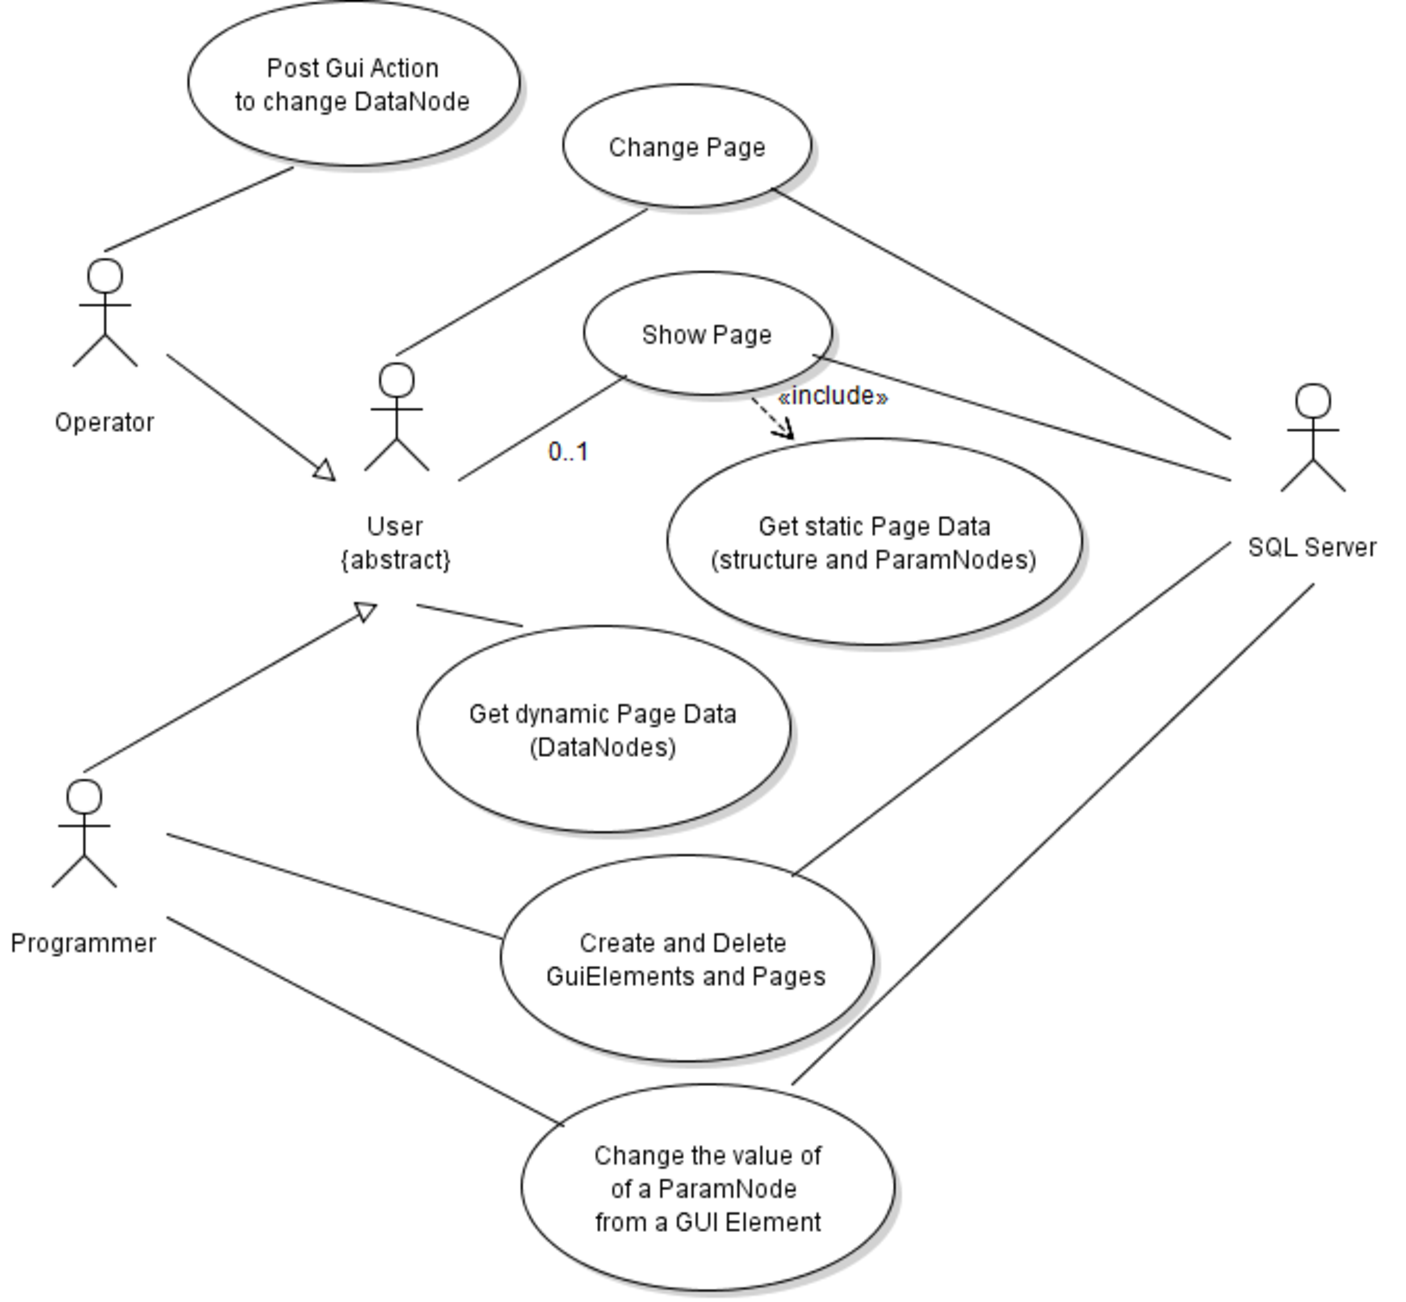
\includegraphics[width=\textwidth]{content/hauptteil/systemEntwurf/res/useCase/I.pdf}
  \caption[Anwendungsfalldiagramm des \acs{scada} Systems I]{Anwendungsfalldiagramm des \acs{scada} Systems I}
  \label{fig:UCI}
\end{figure}
Aus der Zielsetzung der Arbeit ergeben sich die Anwendungsfalldiagramme in Abbildungen \ref{fig:UCI} und \ref{fig:UCII}.
Das Diagramm in Abbildung \ref{fig:UCI} beschreibt abstrakt die Anwendungsfälle, die das \ac{scada} System für den Anwender, in der Rolle des Bedieners (Operator), 
sowie des Programmierers (Programmer) erfüllen muss.
Analog dazu beschreibt das Anwendungsfalldiagramm in Abbildung \ref{fig:UCII} die Anwendungsfälle die ein \ac{plc} an das \ac{scada} System stellt.
Es ist möglich dies in zwei getrennten Diagrammen abzuhandeln, da es keine Anwendungsfälle gibt, die einen Akteur aus beiden Diagrammen benötigt.
Jedoch interagieren alle Akteure mit dem selben System.
%Das A beschreiben %Ein \emph{Operator} muss eine \ac{gui} Aktion an das \ac{scada} übermitteln können. 
%Das ist zum Beispiel das Klicken auf einen Button.

